\documentclass[letterpaper, 10 pt, conference]{sty/ieeeconf}

\IEEEoverridecommandlockouts

\overrideIEEEmargins

\usepackage{graphics}
\usepackage{epsfig}
\usepackage{amsmath}
\usepackage{amssymb}
\usepackage{txfonts}
\usepackage{tikz}
\usepackage{sty/tkz-base}
\usepackage[T1]{fontenc}

\usetikzlibrary{shapes,decorations,shadows}
\usetikzlibrary{decorations.pathmorphing}
\usetikzlibrary{decorations.shapes}
\usetikzlibrary{fadings}
\usetikzlibrary{patterns}
\usetikzlibrary{calc}
\usetikzlibrary{decorations.text}
\usetikzlibrary{decorations.footprints}
\usetikzlibrary{decorations.fractals}
\usetikzlibrary{shapes.gates.logic.IEC}
\usetikzlibrary{shapes.gates.logic.US}
\usetikzlibrary{fit,chains}
\usetikzlibrary{positioning}
\usepgflibrary{shapes}
\usetikzlibrary{scopes}
\usetikzlibrary{arrows}
\usetikzlibrary{backgrounds}
\tikzset{latent/.style={circle,fill=white,draw=black,inner sep=1pt, 
minimum size=20pt, font=\fontsize{10}{10}\selectfont},
obs/.style={latent,fill=gray!25},
const/.style={rectangle, inner sep=0pt},
factor/.style={rectangle, fill=gray!25,minimum size=15pt, inner sep=1pt,draw=black},
>={triangle 45}}

\DeclareMathOperator*{\argmax}{arg\,max}
\DeclareMathOperator*{\argmin}{arg\,min}

\begin{document}

\title{\LARGE \bf
Curb Detection for a Pedestrian Robot in Urban Environments
}

\author{
\authorblockN{
J\'{e}r\^{o}me Maye,
Ralf Kaestner,
and Roland Siegwart}
\authorblockA{
Autonomous Systems Lab, ETH Zurich, Switzerland\\
email: \{jerome.maye, ralf.kaestner, roland.siegwart\}@mavt.ethz.ch}
}

\maketitle

\begin{abstract}
This paper presents a novel ...

\end{abstract}

\section{Introduction}
Urban areas are highly complex environments which introduce numerous challenges
to autonomous service robots. In particular, for a safe and reliable navigation,
a robot should be able to accurately detect curbs. Curbs usually appear at the
borders between streets and sidewalks. The knowledge of curb positions and
characteristics can beneficially enhance metric maps with traversability
information relevant to navigation. For instance, depending on its physical
capabilities, a robotic platform could only drive harmlessly over curbs of a
given height when crossing a street.

Amongst the difficulties related to this task, curbs might exhibit various
curvatures and heights, and be perceived from different viewpoints. In contrast
to autonomous cars, pedestrian robots can indeed make few assumptions about
the structure of the environment. Furthermore, the sensing device noise model
should be introduced to distinguish between real curbs and measurement noise.
Ideally, the algorithm should run on-line and in real-time.

In this paper, we devise an unsupervised method to curb detection that covers
most of the aforementioned requirements. Our approach attempts to construct a
piecewise planar model of the environment and determines curbs at plane segment
boundaries. Initially, we sense the environment with a nodding laser
range-finder and project the 3D measurements into an efficient Digital Elevation
Map (DEM). Each cell of the DEM maintains an error model that is propagated
throughout the entire algorithm. Plane segments are further estimated with a
mixture of linear regression model. Here, we propose an original formulation of
the standard Expectation-Maximization (EM) algorithm for mixture models.
Specifically, in the E-step, the responsibilities are computed with a
Conditional Random Field (CRF) that introduces dependencies between the
covariates of the mixture model. A graph-based segmentation of the DEM provides
an estimate of the number of planes and initial parameters for the EM.
Sequential and fast estimations of DEM patches in the surrounding of the sensor
while the robot drives ensure on-line operation. Fig.~\ref{fig:intro} shows a
typical output of our algorithm with the curb points reprojected on the original
data.

\begin{figure}[t]
\centering
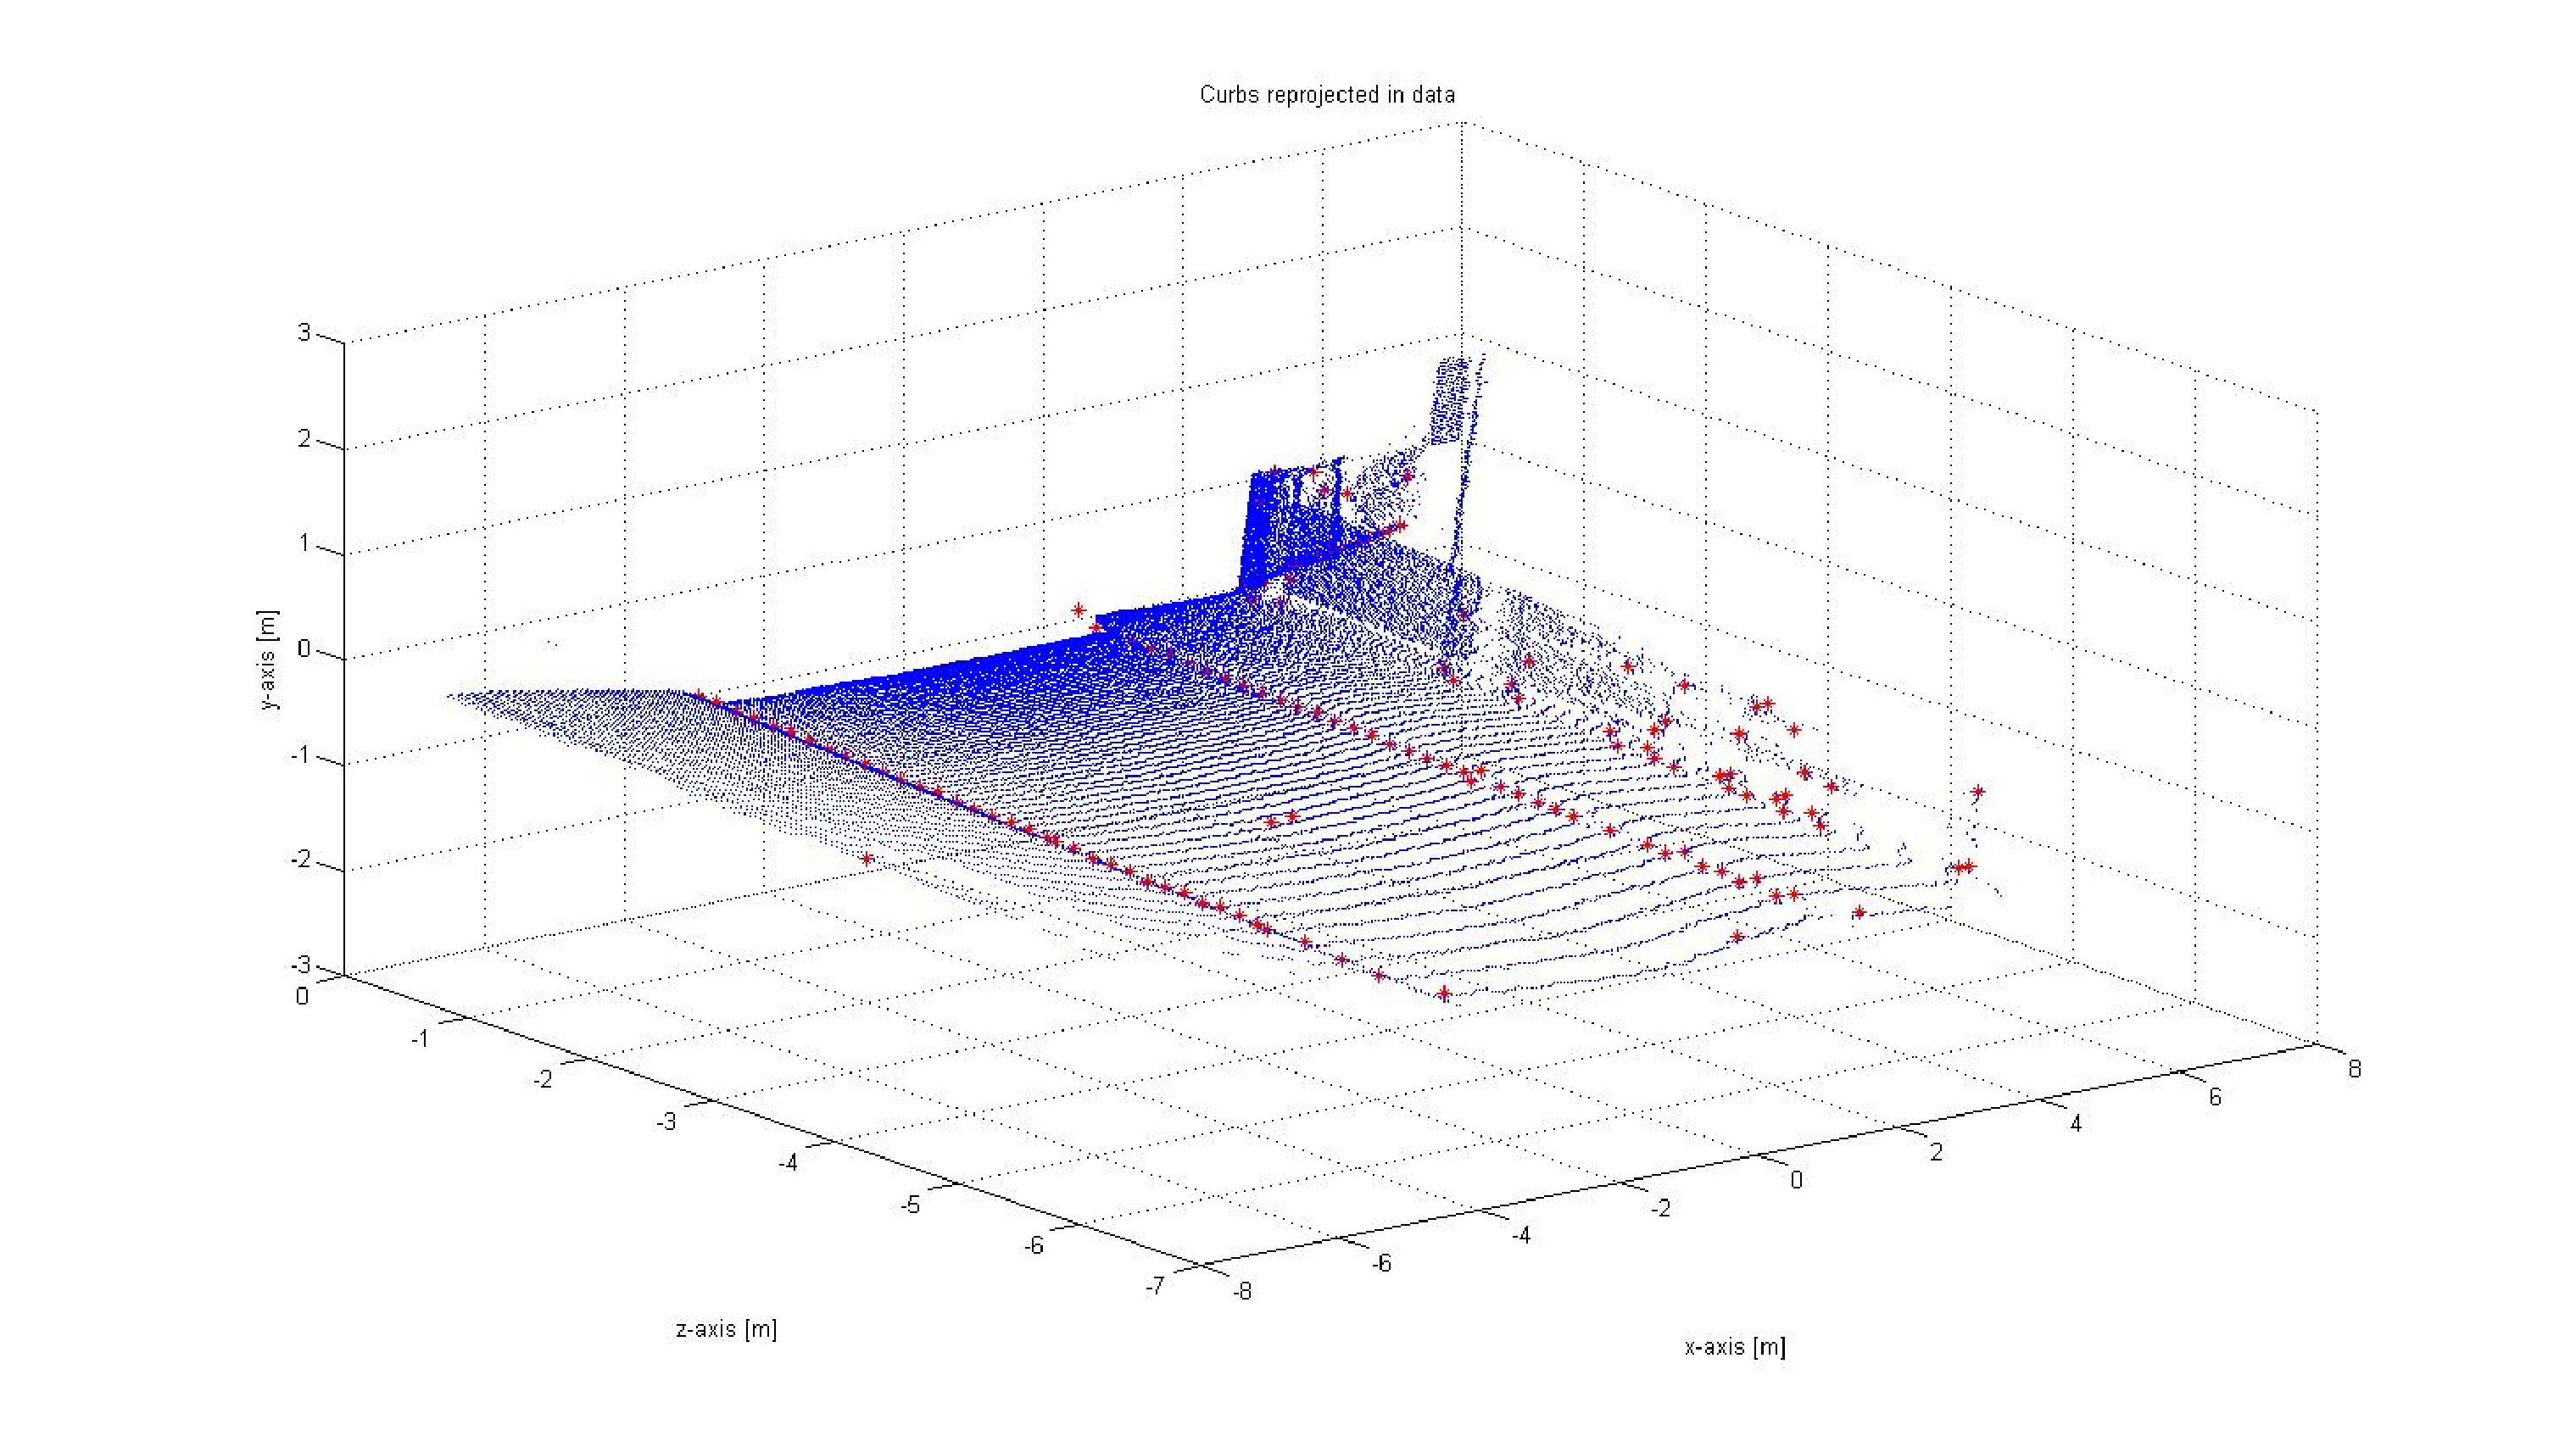
\includegraphics[width=\columnwidth]{fig/intro.eps}
\caption{Exemplary output of our curb detection algorithm. Curb points
(red stars) are reprojected into the original point cloud.}
\label{fig:intro}
\end{figure}

Clearly, the main contribution of the paper is its strict probabilistic
interpretation from the sensing process to the final plane estimation and
segmentation. Moreover, our method is view-independent and requires no
particular prior knowledge about the environment. The set of free parameters
is solely related to the sensor characteristics and involves no hand-tuning.
Finally, a direct implementation of the algorithm from the paper should be
straightforward.

The remainder of the paper is structured as follows. Section~\ref{sec:related}
summarizes the previous works related to ours. Section~\ref{sec:model}
introduces our statistical models and derives the related inference methods.
Section~\ref{sec:implementation} is concerned with implementation and
algorithmic details. Section~\ref{sec:exp} demonstrates the validity of the
method through extensive qualitative and quantitative analysis.
Section~\ref{sec:conc} outlines our conclusions and provides some insights for
future work.


\section{Related Work\label{sec:related}}
The problem of curb or \emph{step} detection has mainly been studied in the
context of Intelligent Transportation Systems (ITS), covering an extensive set
of sensing modalities and algorithms. In ITS, one might assume a typical
experimental setting where a car drives on a street and curbs are situated on
the left and right side of the vehicle. Therefore, most of these approaches
are inappropriate as such for a pedestrian robot navigating in cities. In this
situation, curbs will indeed appear under multiple viewpoints. We hence review
the main influential contributions to the field and relate them to our method.

In~\cite{oniga10polynomial}, Oniga \emph{et al.} employ a dense stereo-vision
system to capture a 3D point cloud, which is further transformed into a Digital
Elevation Map (DEM). Curbs are represented as third-order polynomials. Candidate
curb points are extracted with a Canny edge detector. A RANdom SAmple Consensus
(RANSAC) polynomial fitting is then applied to perform outlier rejection and
find the polynomial coefficients. The location of the curbs and their heights
are finally obtained with some further refinement steps. In comparison to this
method, we use the same measurement representation (DEM). However, we draw a
clear and sound probabilistic model from the sensing device to the curb
detection and limit the number of hand-tuned parameters.

Closer to our approach, Siegemund \emph{et al.}~\cite{siegemund10curb} proposed
a promising method that extracts curbs from dense stereo-vision data. We
actually take inspiration on their ideas and solve their major drawbacks. In
this paper, as mentioned above, they assume a strict environment model and they
lack a unified probabilistic model. Moreover, their curb models can only
represent a limited set of curbs. For instance, they cannot model T
junctions or roundabouts.

In~\cite{shin10drivable}, Shin \emph{et al.} use a similar setup as ours, i.e.,
a mobile robot equipped with a laser range-finder. They however stick to a
restricted environment model and their tilted laser only provides a single laser
line. Their algorithm is mostly engineered to fit their particular application
and setup, and again does not build on sound probabilistic model.

An alternative application of step detection is presented
in~\cite{pradeep08piece}. In this paper, Pradeep \emph{et al.} aim at mobility
aids for visually impaired people, as a complement to the white cane or the dog.
This naturally imposes restrictions in the sensing device, in this case a
wearable and cheap stereo camera. Their curb detection algorithm is based on the
same motivation as ours, i.e., building a piecewise planar model of the scene.
In their implementation, point-wise normal vectors are firstly estimated with
Principal Component Analysis on a local neighborhood and RANSAC for outlier
rejection. Tensor voting is then applied for finding globally consistent plane
normals and a final clustering step extracts the plane segments. Although it
solves many of the above issues, this method might also suffer from the lack of
any underlying probabilistic models.

In~\cite{yuan05dynamic}, Yuan and Manduchi also developed an algorithm for
visually impaired people, working with a custom sensing device called
a "Virtual White Cane". Their method uses a Jump-Markov Process to detect
geometric singularities in the range measurements. Despite its statistical
foundations, it will not generalize well to our application requirements and
provide a plane estimation.


\section{Model\label{sec:model}}
\subsection{Measurements Representation}
Scan measurements $\mathbf{s}_i=[r_i,\theta_i,\psi_i]^\text{T}$ are transformed
into their corresponding Cartesian 3D coordinates $\mathbf{p}_i=[x_i,y_i,z_i]
^\text{T}$, where $r_i$ is a range measurement, $\theta_i$ a pitch angle, and
$\psi_i$ a bearing angle. From a complete laser sweep, we obtain a point cloud
representation $\mathcal{P}=\{\mathbf{p}_1,\mathbf{p}_2,\dots,\mathbf{p}_N\}$.
$\mathcal{P}$ is finally projected onto a 2D grid $\mathcal{G}=\{\mathcal{C}_1,
\mathcal{C}_2,\dots,\mathcal{C}_M\}$, with cells $\mathcal{C}_i=
\{\mathbf{ul}_i,\mathbf{lr}_i,\mathbf{c}_i,h_i,l_i,\mathcal{I}_i\}$, where
$\mathbf{ul}_i$ and $\mathbf{lr}_i$ are the upper left and lower right 2D
coordinates of the cell, $\mathbf{c}_i$ the center of the cell, $h_i$ the height
of the cell such that $h_i\propto\mathcal{N}(\mu_i,\sigma_i)=p(h_i\mid\mu_i,
\sigma_i,\mathcal{I}_i)$, $l_i\in\{1,\dots,M\}$ a discrete label for the cell,
and $\mathcal{I}_i=\{\mathbf{p}_j\mid\mathbf{p}_j\in\mathcal{P},
\mathbf{p}_{j_x}>\mathbf{ul}_{i_x},\mathbf{p}_{j_y}>\mathbf{ul}_{i_y}
,\mathbf{p}_{j_x}<\mathbf{lr}_{i_x},\mathbf{p}_{j_y}<\mathbf{lr}_{i_y}
,\mathbf{p}_{j_z}<\theta_U,\mathbf{p}_{j_z}>\theta_L\}$. $\theta_U$
and $\theta_L$ define upper and lower bounds for the height values.

The grid $\mathcal{G}$ will also be referred to as a Digital Elevation Map (DEM)
in the rest of the paper. The choice of a DEM representation is mainly guided by
the final outcome of the algorithm, i.e. a traversability map for the planning
process. It is also convenient for defining Regions of Interest (ROI) in
$\mathcal{P}$ and for simplifying the subsequent computations. We could also
have resorted to a polar grid representation, so as to have a finer resolution
close to the sensor (THIS IS STILL OPEN AND NEED FURTHER EXPLANATIONS). Whenever
the number of points in a cell $\mathcal{C}_i$ is below a threshold, i.e.
$|\mathcal{I}_i|<\theta_P$, it is flagged as invalid.

REMARKS:
\begin{itemize}
\item EXPLAIN HOW WE CAN GO FROM THE PUSH-BROOM LASER DATA TO THE DEM
\item EXPLAIN WHAT HEIGHT $h_i$ IS FINALLY TAKEN
\end{itemize}

\subsection{Environment Model and Inference Task}
We assume a piecewise planar environment, i.e., the observed scene is composed
of a set of plane segments $\mathcal{S}_1,\mathcal{S}_2,\dots,\mathcal{S}_M$, with
$\mathcal{S}_i=\{\mathcal{C}_j\mid h_j=\mathbf{w}_i^\text{T}\boldsymbol{\phi}
(\mathbf{c}_{j})\}$, $\mathbf{w}_i=[w_0^{(i)}, w_1^{(i)}, w_2^{(i)}]^\text{T}$,
and $\boldsymbol{\phi}(\mathbf{c}_{j})=[1,\mathbf{c}_j]^\text{T}$.

Boundaries between plane segments define local heights discontinuities that we
shall term \emph{curbs} from now on. The major inference task therefore boils
down to discovering those plane segments. To this end, we follow a probabilistic
and iterative approach.


\section{Implementation Details\label{sec:implementation}}
\subsection{Initial Estimates and Model Complexity}

The number of mixture components $k$ in Equ.~\eqref{eqn:mixture} and initial
responsibilities have to be specified for computing the regression parameter set
$\Theta^\text{old}$ and for running the CRF framework. For this purpose, we
adopt the graph-based algorithm from Felzenzswalb and
Huttenlocher~\cite{felzenszwalb04efficient}. Although this method was originally
designed for image segmentation, we can adapt it for our intent, by treating
image regions as plane segments.

We hence define an undirected graph $\mathcal{G}=\{\mathcal{V},\mathcal{E}\}$,
with vertices $v_i\in\mathcal{V}$ to be segmented and edges $(v_i,v_j)
\in\mathcal{E}$ connecting neighboring vertices. Each edge has a weight
$w((v_i,v_j))$ proportional to the dissimilarity between $v_i$ and $v_j$. In our
particular setting, a valid grid cell $\mathcal{C}_i$ is aligned with a
vertex $v_i$ and each vertex has a 4-connected neighborhood. The goal of the
algorithm is to find a partition of $\mathcal{V}$ into segments $\mathcal{S}_i$
that correspond to the connected components of a graph
$\mathcal{G}'=\{\mathcal{V},\mathcal{E}'\}$, with $\mathcal{E}'\subseteq
\mathcal{E}$. We are interested in the specific
partition such that vertices in a component have a high similarity and vertices
in different components a low similarity. Therefore, edges between vertices in
the same component should have a low weight and edges between vertices in
different components a high weight. The weight function can be described with
the symmetric Kullback-Leibler divergence between two cells, i.e.,
$w((v_i,v_j))=D_{KL}(h_i\mid\mid h_j)+D_{KL}(h_j\mid\mid h_i)$. We thus take
into account the full height distributions, in particular the variances. For
normal distributions, the Kullback-Leibler divergence integrates analytically to

\begin{equation}
\label{eqn:kl}
D_{KL}(h_i\mid\mid h_j)=\frac{(\mu_{h_i}-\mu_{h_j})^2}{2\sigma_{h_j}^2}+
\frac{1}{2}(\frac{\sigma_{h_i}^2}{\sigma_{h_j}^2}-1-\ln\frac{\sigma_{h_i}^2}
{\sigma_{h_j}^2}).
\end{equation}

The algorithm starts with all vertices belonging to a different component. It
then iterates over the set of edges ordered by increasing weights. For each
edge $(v_i,v_j)\in\mathcal{E}$ with $v_i\in\mathcal{S}_k$,
$v_j\in\mathcal{S}_l$, and $\mathcal{S}_k\neq\mathcal{S}_l$, the two components
are merged if

\begin{equation}
\label{eqn:merge}
w((v_i,v_j))\leq MInt(\mathcal{S}_k, \mathcal{S}_l),
\end{equation}


where $MInt(\mathcal{S}_k,\mathcal{S}_l)=\min(Int(\mathcal{S}_k)+
\tau(\mathcal{S}_k),Int(\mathcal{S}_l)+\tau(\mathcal{S}_l))$,
$Int(\mathcal{S})=\max_{(v_i,v_j)\in\mathcal{S}} w((v_i,v_j))$, and
$\tau(\mathcal{S})=s/|\mathcal{S}|$. Two components should be disconnected if
the difference between them is large compared to the internal difference within
at least one of the components. $s$ is a scale parameter that controls the
preference for larger components. The algorithm runs in $O(n\log n)$, where
$n=|\mathcal{E}|$.

Although the algorithm does not convey any probabilistic interpretation in the
resulting segmentation, we transform the hard assignment of a grid cell
$\mathcal{C}_i$ to a component $\mathcal{S}_k$ into the following discrete
distribution:

\begin{equation}
\label{eqn:label_dist}
p(l_i=k) = \left\{
\begin{array}{l l}
1 & \quad \text{if $\mathcal{C}_i\in\mathcal{S}_k$}\\
0 & \quad \text{otherwise}.
\end{array} \right.
\end{equation}

\subsection{Missing Data}

\subsection{Algorithmic Complexity}




\section{Experiments\label{sec:exp}}
In order to evaluate the approach proposed in this paper, ...


\section{Conclusion\label{sec:conc}}
In this paper, we have presented a novel approach to curb detection. We have
devised an unsupervised method that is applicable to various environment
configuration and perspective views. We have demonstrated an application to a
pedestrian robot and shown the robustness of our approach through a thorough
experimental evaluation on real-world and synthetic data.

From a theoretical point of view, we have anchored our method to sound
statistical models from the measurement process to the final inference tasks.
This results into an elegant and efficient algorithm that is solely
parameterized by sensor characteristics. Our approach reconstructs the
environment as a mixture of plane segments and flags curbs at their boundaries.
For the parameter estimation, we have replaced the standard E-step of the
Expectation-Maximization (EM) algorithm with loopy Belief Propagation (BP) and
justified its utilization. Finally, we have tackled model selection issues with
a graph-based segmentation heuristic.

As a future work, we envision to apply a fully Bayesian treatment to our
method and investigate the use of Hierarchical Mixture of Experts
(HME)~\cite{jordan94hierarchical,bishop03bayesian}. Additionally, we want to
study the feasibility of a recursive estimation framework. Since BP is amenable
to parallelization, it would also be beneficial to use a GPU implementation.


\section*{Acknowledgment}
This work has partly been supported by the EC under FP7-231888-EUROPA.
\vspace{6.3mm}
\bibliographystyle{sty/IEEEtran}
\bibliography{bib/bibliography}

\end{document}
